\chapter{Theoretische Grundlagen}

-> Nur Theorie, die später auch verwendet wird, nichts einfach so einführen

-> Voraussetzung: Basiswissen WI-Studium

\section{Geschäftsprozessanalyse und Prozessoptimierung}

-> Allgemeine Theorie zur Geschäftsprozessanalyse und Prozessoptimierung (wenn passende Literatur vorhanden auch direkt in Verbindung mit Massendaten-Management)

-> Darstellung von Methoden/ Frameworks zur Prozessanalyse, -optimierung

\section{User Experience im Geschäftsprozesskontext}

-> Literatur zu UX (allg., Massendaten-Management-Kontext, Business-Software-Kontext)

\section{Massendaten-Management}

-> allgemeine Theorie hinter effizientem Massendaten-Management erläutern (Anlage, Verwaltung, Änderung, Löschung)

\section{SAP Produkte}

\subsubsection{SAP Ariba Direct Materials Sourcing for Automotive and Industrial Manufacturing in SAP S/4 HANA}

Die ''SAP Ariba Direct Materials Sourcing for Automotive and Industrial Manufacturing in SAP S/4 HANA''-Suite (im Folgenden mit ''DMS'' abgekürzt) ist ein Lösungs-Portfolio in der Cloud für die direkte Beschaffung in der Automobilindustrie und im produzierenden Gewerbe. Beschaffung meint in diesem Kontext strategische Handlungsfelder des Einkaufs. Solche sind \zB die Marktforschung, Lieferantenauswahl, Vertragsverhandlungen und Risikomanagement. \footcite[Vgl.][S. 541]{theorie_digitale_transformation_beschaffung_automobilindustrie_2019} Direkte Beschaffung bezeichnet den Einkauf von Gütern, die direkt in die Herstellung des Produkts eingehen, während indirekte Beschaffung den Einkauf von Gütern, die die Produktion unterstützen, beschreibt. \footcite[Vgl.][S. 541]{theorie_digitale_transformation_beschaffung_automobilindustrie_2019} Die DMS-Suite ist speziell für die Automobil- und Fertigungsindustrie konzipiert, da diese Branchen mit komplexen Produktionsprozessen und Bauteilen arbeiten und die Kooperation mit Lieferanten bei der Entwicklung neuer Produkte von gro\ss er Bedeutung ist. Mit S/4 HANA (im Folgenden mit ''S/4'' abgekürzt) als Basis kann gesamten Lebenszyklus der Bauteile, von der Produktentwicklung über die Beschaffung bis zum Qualitätsmanagement, abgedeckt werden. Das ermöglicht Kosteneinsparungen durch Effizienzsteigerung und ermöglicht ein transparentes Reporting des CO2-Fu\ss abdrucks. Zudem können alle Produkte durch das einheitliche Datenmodell einfach verknüpft werden. Durch die Vernetzung der Lösungen stehen alle Beschaffungsdaten in jedem System zur Verfügung und verbessern Entscheidungsfindung und Transparenz. \footcite[Vgl.][]{theorie_sap_webseite_dms_übersicht_2024}

\begin{figure}[H]
    \centering
    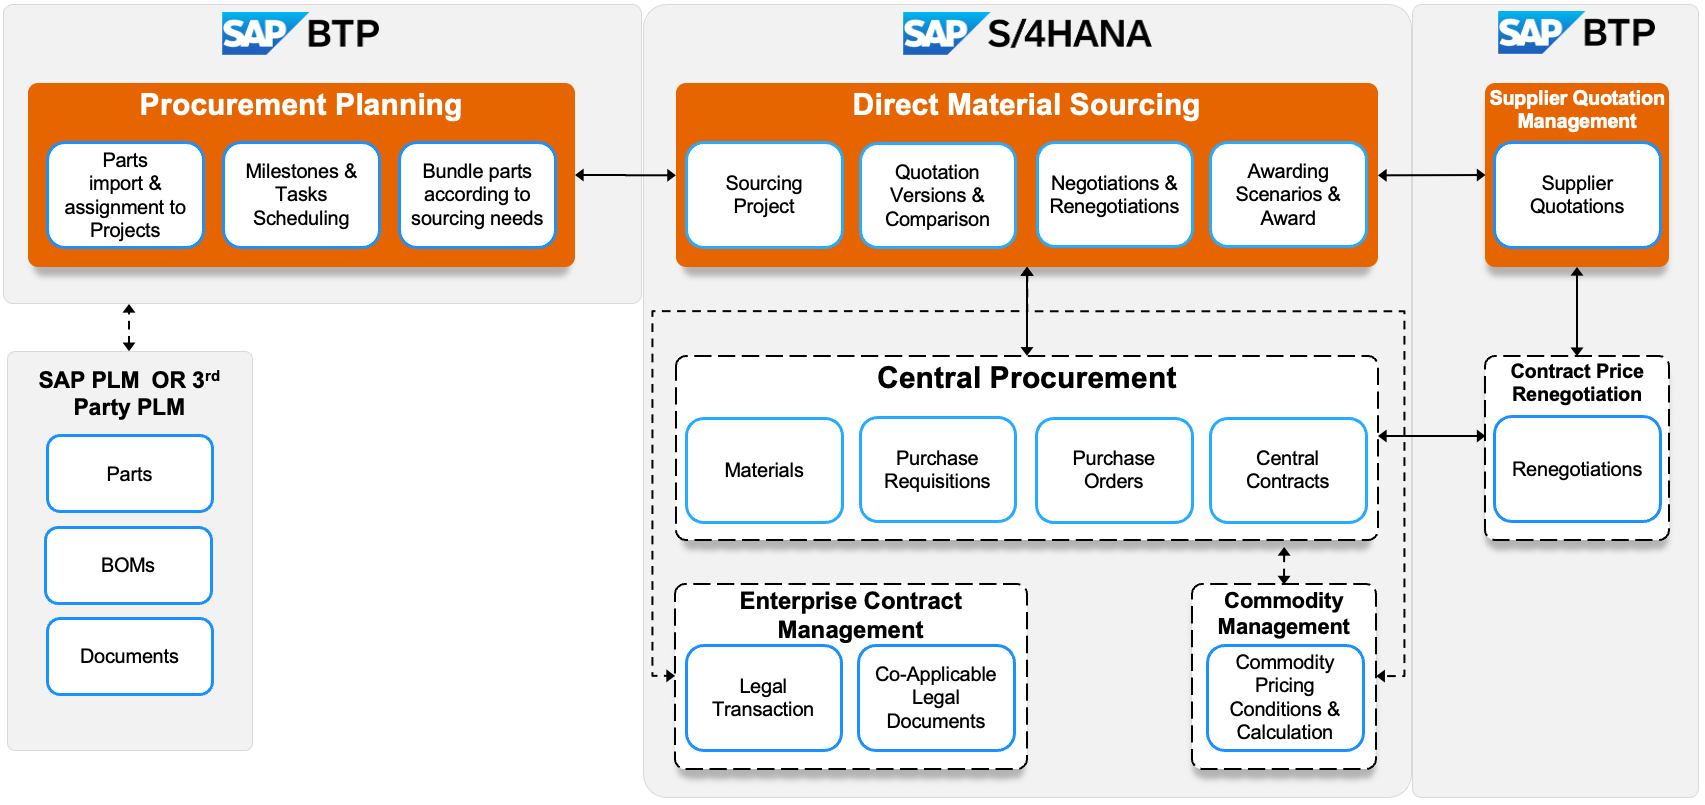
\includegraphics[height=7.1cm]{Bilder/Direct_Material_Sourcing_Overview3.png}
    \caption[SAP Ariba DMS Suite Produktübersicht]{SAP Ariba DMS Produktübersicht. Eigene Darstellung}
    \label{fig:iso_norm}
\end{figure}

Im Folgenden werden die einzelnen Bestandteile der Suite beschrieben: Der Kern des Portfolios besteht aus den Produkten Procurement Planning, Direct Material Sourcing und Supplier Quotation Management. Optional kann vor Procurement Planning ein Product Lifecycle Management System von SAP oder einem Drittanbieter (im Folgenden ''PLM'' abgekürzt) integriert werden. In diesem System wird der gesamte Lebenszyklus des Produkts, von der Idee bis zum Support verwaltet. In diesem Kontext ist die Entwicklung von Bauteilen des Produkts und die Kollaboration mit Lieferanten relevant. \footcite[Vgl.][]{theorie_sap_plm_übersicht_2024} Aus dem PLM-System werden dann die benötigten Teile mit Spezifikationen in Procurement Planning übertragen. In Procurement Planning werden dann aus diesen Teile-Listen Beschaffungsprojekte erstellt. Innerhalb dieser Projekte wird der Bedarf und die dafür nötigen Finanzmittel über die Produktionsspanne des Produkts geplant. Durch das Setzen verschiedener Ziel-Daten werden Meilensteine rückwirkend geplant, sodass die Beschaffung anhand des Produktionsplans rechtzeitig erfolgt. \footcite[Vgl.][]{theorie_sap_procurement_planning_overview_2024} Nach der Planung, welche Mengen der verschiedenen Teile benötigt werden, werden diese in Beschaffungsprojekte gruppiert und in die Software Direct Material Sourcing übertragen. In diesem Schritt findet der eigentliche Einkauf statt. Die benötigten Bauteile werden ausgeschrieben und Lieferanten können in einem mehrstufigen Verfahren Angebote abgeben, bis dann nach mehreren Verhandlungsrunden ein Lieferant den Zuschlag erhält. \footcite[Vgl.][]{theorie_sap_webseite_dms_übersicht_2024} Die Verwaltung und Abgabe der Lieferantenangebote wird durch das Produkt Supplier Quotation Management unterstützt. Auf dieser Plattform können Lieferanten offene Ausschreibungen einsehen und Angebote abgeben. \footcite[Vgl.][]{theorie_sap_supplier_quotation_management_help_2024} Da viele Automobil- und Fertigungsunternehmen ihre Beschaffungsorganisation zentralisieren, kann Direct Material Sourcing mit dem Produkt Central Procurement verknüpft werden. Dadurch kann die Beschaffung über mehrere Standorte hinweg zentral gesteuert werden. Diese Lösung wird im nächsten Kapitel noch genauer beschrieben. Die Erstellung und Verwaltung legaler Verträge mit Lieferanten wird durch das Enterprise Contract Management unterstützt. Einkäufer können in Zusammenarbeit mit der Rechtsabteilung Verträge anhand von Vorlagen erstellen und zentralisiert verwalten. \footcite[Vgl.][]{theorie_sap_enterprise_contract_management_2024} Da viele Bauteile in der Industrie rohstoffintensiv sind, ist es möglich über das Produkt Commoditiy Management indexbasiert Preise für Rohstoffe mit den ausgeschriebenen Produkten zu verknüpfen, um Preisschwankungen abzufedern und daraus resultierende finanzielle Risiken zu minimieren. \footcite[Vgl.][]{theorie_sap_commodity_management_2024} Zuletzt ist noch die Lösung Contract Price Renegotiation zu nennen, durch die langfristige Verträge mit Lieferanten in festen Intervallen neu verhandelt werden können, um Preisänderungen, Effizienzsteigerungen und Skaleneffekten Rechnung zu tragen. Dadurch können für den Einkauf durch günstigere Kostenstrukturen Einsparungen erzielt werden. \footcite[Vgl.][]{theorie_sap_contract_price_renegotiation_2024}

\subsubsection{SAP Ariba Central Procurement}

SAP Ariba Central Procurement (im Folgenden ''CP'' abgekürzt) ist ein Produkt der DMS-Suite, welches die Zentralisierung der Beschaffung in einem Unternehmen ermöglicht. Gro\ss e Konzerne im Automobilsektor oder der Industrie haben meistens weltweit Tochtergesellschaften und Standorte mit jeweils eigenen IT-Systemen und Prozessen. Durch die Zentralisierung der Beschaffung können diese Prozesse vereinheitlicht und die IT-Systeme vernetzt werden. Durch die zentrale Steuerung der Beschaffungsorganisation werden Ineffizienzen vermieden, Kosten gespart und die Transparenz erhöht. Globale Richtlinien lassen sich einfacher durchsetzen und die Verhandlungsmacht gegenüber Lieferanten steigt durch gebündelte Bestell-Volumina. \footcite[Vgl.][]{theorie_sap_central_procurement_overview_2024}

\begin{figure}[H]
    \centering
    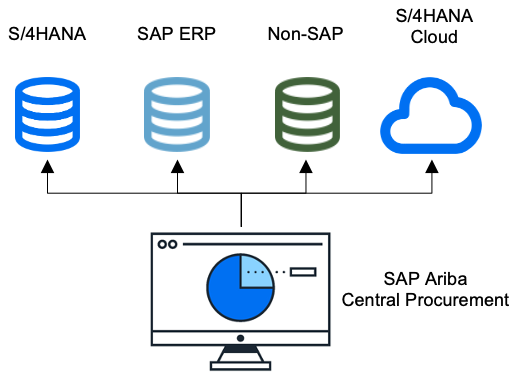
\includegraphics[height=6cm]{Bilder/Central_Procurement_System_Landscape.png}
    \caption[SAP Ariba Central Procurement Systemlandschaft]{SAP Ariba Central Procurement Systemlandschaft. Eigene Darstellung}
    \label{fig:iso_norm}
\end{figure}

In einer bestehenden Systemlandschaft eines Unternehmens nimmt das CP-System die Rolle eines ''Hub''-Systems ein, das mit allen lokalen ERP-Systemen der einzelnen Standorte verbunden wird. Diese Systeme können SAP-Lösungen oder Systeme von Drittanbietern sein. Alle Beschaffungsdaten der lokalen Systeme sind in CP verfügbar und sind in beide Richtungen synchronisiert. CP besteht aus vier Sub-Lösungen: Central Requisitioning, Central Purchasing, Central Sourcing und Central Contracts. Central Requisitioning ermöglicht  das Sammeln aller Bestellanfragen der Standorte. Dadurch erhalten Einkäufer einen Überblick über den globalen Bedarf an bestimmten Teilen und können diesen gesammelt bei bestimmten Lieferanten beschaffen. Central Purchasing deckt diese Beschaffung ab, indem alle Bestell-Anforderungen eines Bauteils gesammelt in einer Ausschreibung beschafft werden können. Durch Central Sourcing kann die Lieferantenauswahl zentral nach strategischen Gesichtspunkten gesteuert werden und so das Lieferkettenrisiko minimiert werden. Durch Central Contracts können mit den ausgewählten Lieferanten langfristige Verträge geschlossen werden, die den Rahmen der Kooperation und Bedarfs-Mengen für mehrere Jahre festlegen. Diese als Basis für konkrete Bestellungen aus den lokalen Systemen und alle Einkäufer der unterschiedlichen Tochtergesellschaften profitieren von den zentral verhandelten Konditionen. Des weiteren bietet CP Analyse- und Reportingfunktionalitäten, um die Beschaffungsprozesse auf globaler Ebene zu überwachen und Optimierungspotenzial zu identifizieren. \footcite[Vgl.][]{theorie_sap_central_procurement_overview_2024}

\subsubsection{Central Contracting}


% -> Central Contracts (Was stellt das Objekt im Prozess dar, wie wird es genutzt, welche Daten werden dort abgelegt?, ...)